\documentclass[conference, table]{IEEEtran}
\IEEEoverridecommandlockouts

\usepackage{cite}
\usepackage{amsmath,amssymb,amsfonts}
\usepackage{graphicx}
\usepackage{textcomp}
\usepackage{xcolor}

% own packages
\usepackage{url}
\usepackage{tabularx}
\usepackage{makecell}
\usepackage{multirow}
\usepackage{booktabs}
\usepackage{caption}
\usepackage{stfloats}
\usepackage{tikz}
\usetikzlibrary{arrows.meta, positioning, fit, calc, backgrounds}
\usepackage{hyperref}
\usepackage{orcidlink}

\newcommand{\fsixteen}{F16}
\newcommand{\qfour}{Q4\_K\_M}

\def\BibTeX{{\rm B\kern-.05em{\sc i\kern-.025em b}\kern-.08em
    T\kern-.1667em\lower.7ex\hbox{E}\kern-.125emX}}
\begin{document}

\title{The Graph Changes, the Answers Don't: 4-Bit Quantization in Knowledge-Graph RAG}

\author{
    \IEEEauthorblockN{
        Mirza Shahzaib Baig\,\orcidlink{0009-0008-0944-4413}\IEEEauthorrefmark{1},
        Tobias Deu{\ss}er\IEEEauthorrefmark{1}\IEEEauthorrefmark{2},
        Lorenz Sparrenberg\IEEEauthorrefmark{1}\IEEEauthorrefmark{2}\IEEEauthorrefmark{3},
        Rafet Sifa\IEEEauthorrefmark{1}\IEEEauthorrefmark{2}\IEEEauthorrefmark{3}
    }
    \IEEEauthorblockA{\IEEEauthorrefmark{1} Institute of Computer Science, University of Bonn, Bonn, Germany}
    \IEEEauthorblockA{\IEEEauthorrefmark{2} Lamarr Institute for Machine Learning and Artificial Intelligence, Bonn, Germany}
    \IEEEauthorblockA{\IEEEauthorrefmark{3} Fraunhofer IAIS, Sankt Augustin, Germany}
    \texttt{s42mbaig@uni-bonn.de}
    \thanks{This research has been funded by the Federal Ministry of Education and Research of Germany and the state of North-Rhine Westphalia as part of the Lamarr-Institute for Machine Learning and Artificial Intelligence.}
}

\maketitle

\begin{abstract}
Quantizing the generator of a knowledge-graph RAG (KG-RAG) pipeline substantially changes the knowledge graph it builds while leaving the answers it produces intact, and this paper establishes why. KG-RAG invokes the generator twice, once to \emph{extract} a graph from the corpus at index time and once to \emph{answer} from it at query time, so reduced precision can degrade quality through a channel that standard benchmarks never probe: a damaged graph that handicaps every later query. We isolate that channel with a controlled paired experiment in LightRAG, holding the documents, chunking, embedder, retrieval mode, decoding parameters and judge fixed and varying only the generator's weight precision (\fsixteen\ versus 4-bit \qfour\ Qwen2.5-7B-Instruct) across 50 indexes, five SQuAD corpus sizes with five seeds each, and 33{,}497 paired questions. The graphs do diverge: exact node overlap is $0.55$--$0.62$ and exact edge overlap $0.23$--$0.27$. Yet judged correctness, pass rate, lexical recall and retrieval Hit@$k$/MRR are indistinguishable, with $|d_z| \leq 0.031$. Two measurements account for the decoupling. Semantic overlap reaches $0.85$ for nodes against $0.62$ exact, so most divergence is surface form; and on the residual, each arm answers $\sim\!0.11/5$ better on questions touching entities only it extracted ($p < 10^{-7}$ in both directions), so the two advantages cancel at corpus level. Quantization \emph{exchanges} extracted knowledge rather than destroying it. With $\sim\!3\times$ less weight memory and up to $2.3\times$ faster index construction, 4-bit is a favourable default for KG-RAG.
\end{abstract}

\begin{IEEEkeywords}
retrieval-augmented generation, knowledge graphs, quantization, large language models, LightRAG, question answering, evaluation
\end{IEEEkeywords}

\section{Introduction}

\noindent
Serving a large language model is expensive. A seven-billion-parameter model held in half precision occupies roughly 15\,GB of accelerator memory before any context or key--value cache is allocated. \emph{Post-training quantization} is the standard remedy, and four bits has emerged as the practical sweet spot: scaling analyses identify 4-bit as near-optimal for a fixed memory budget \cite{dettmers2023case}, and 4-bit formats are the default in the widely used \texttt{llama.cpp} serving stack \cite{llamacpp}. A now-large body of work reports that the accuracy cost is small \cite{ptqsurvey2021,gptq2023,awq2024,quanteval2024}.

\noindent
Separately, retrieval-augmented generation (RAG) has become the standard way to ground a model in an external corpus \cite{rag2020}. Its knowledge-graph variant (KG-RAG) goes further: instead of retrieving raw text alone, the LLM first reads the corpus and extracts a graph of entities and relations, and retrieval then runs over that structure. GraphRAG \cite{graphrag2024} popularized the idea; LightRAG \cite{lightrag2024}, which we study here, keeps the extracted graph but replaces community summarization with a lighter dual-level retrieval scheme.

\noindent
The two developments intersect at a point that neither literature has examined, illustrated in Fig.~\ref{fig:pipeline}. In a KG-RAG pipeline the same generator does two very different jobs. At indexing time it reads every chunk and extracts the entities and relations that become the graph, and at query time it extracts the search keywords and writes the final answer. Quantizing that one model therefore opens two channels through which quality can degrade. The obvious one is generation: a lower-precision model might write worse answers. The less obvious, and arguably the more consequential, one is construction: a lower-precision model might build a worse graph, missing entities, mislabelling them, or dropping relations, and that damaged artefact would handicap retrieval for every query thereafter, no matter how well the model answers. The ``4-bit is nearly lossless'' result was established for standalone generation scored against a benchmark; whether it transfers to a structured artefact the model builds, which then propagates through a multi-stage pipeline, is not obvious.

\noindent
The question falls between three research areas. Quantization research scores what a model says in response to a prompt, not artefacts it produces for something else to consume. RAG evaluation measures end-to-end answer quality and compares retrievers or prompting strategies, without tracing one upstream design choice into the intermediate representation the pipeline builds. KG-RAG research builds and evaluates such pipelines end to end, treating the graph as a means to an answer rather than an object whose fidelity is itself worth measuring. What generator quantization does to the constructed graph, and whether any of it reaches the answers, has to our knowledge not been studied.

\noindent
We close that gap with a controlled paired experiment. For each corpus size and seed, two LightRAG indexes are built over the \emph{identical} documents, differing only in the generator's weight precision: half precision (\fsixteen) against the 4-bit k-quant \qfour. Chunking, the embedding model, the retrieval mode, the decoding parameters and the judge are all held fixed, so any measured divergence is attributable to quantization alone. We propose no new system: both arms are the standard LightRAG pipeline, and the second arm exists to isolate one variable, not to offer an alternative to KG-RAG as it is normally built.

\noindent
The study deliberately covers one generator and one quantization scheme: each (size, seed) cell needs two full index builds and two full evaluation passes, and the 50 indexes and 33{,}497 paired questions reported here already cost several hundred GPU-hours. We spent that budget on depth rather than breadth, and Section~\ref{sec:discussion} returns to what that leaves open. We measure at two levels and relate them, the structure and semantics of the graph and downstream answer and retrieval quality. Our contributions are:

\begin{enumerate}
\item \textbf{The mechanism: quantization \emph{exchanges} extracted knowledge rather than deleting it.} This is the paper's central result. A semantic overlap measure shows most structural drift is surface form, and a targeted probe on the residual, grouping questions by whose exclusive entities they touch, finds a real but \emph{symmetric}, self-cancelling effect, each arm answering better on its own exclusive entities by the same margin. The result explains the decoupling rather than merely observing it, and it predicts where the decoupling would break.
\item \textbf{Evidence that exact structural drift and downstream utility are decoupled.} The graphs disagree substantially by exact overlap (node Jaccard $0.55$--$0.62$, edge Jaccard $0.23$--$0.27$) while the two pipelines are statistically and practically indistinguishable on judged correctness, lexical recall, and retrieval, over 33{,}497 paired questions.
\item \textbf{A multi-seed controlled comparison} that makes both of the above measurable: 50 indexes across five corpus sizes (200--3000 documents) with five seeds each, so every reported difference is accompanied by its run-to-run variability rather than resting on a single build.
\item \textbf{A practical recommendation}, quantified: $\sim\!3\times$ less weight memory and up to $2.3\times$ faster index construction for no measurable quality cost.
\end{enumerate}

\begin{figure*}[t]
\centering
\resizebox{\textwidth}{!}{%
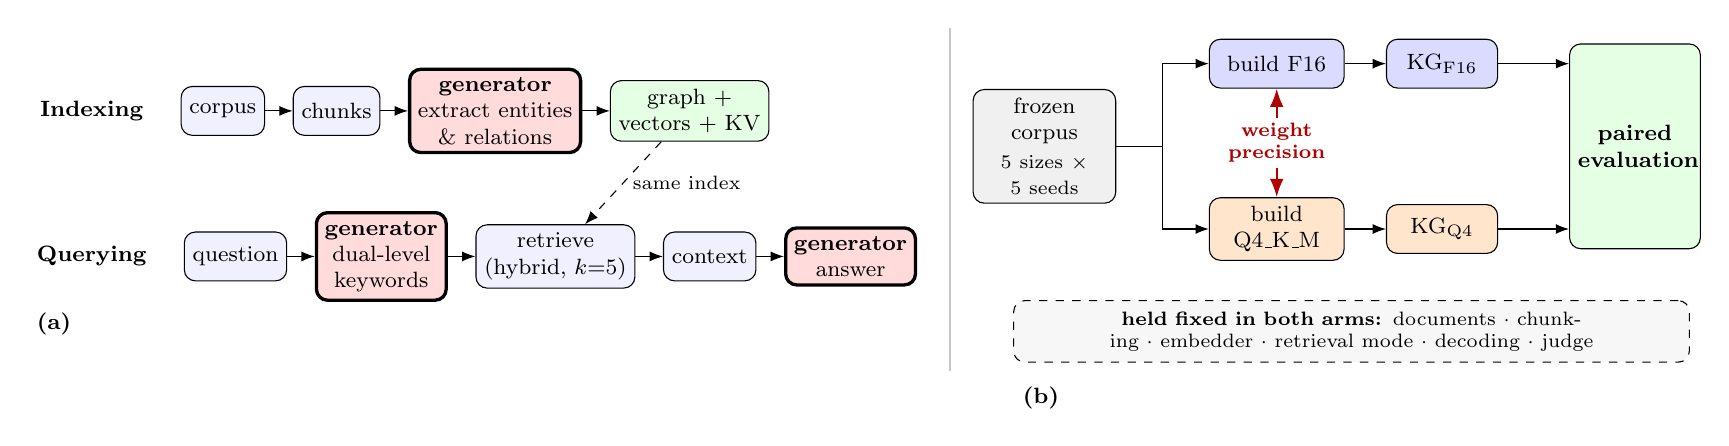
\begin{tikzpicture}[>=Latex, font=\footnotesize,
  b/.style={draw, rounded corners, align=center, minimum height=0.62cm, inner sep=3pt, fill=blue!6},
  llm/.style={draw, rounded corners, align=center, minimum height=0.62cm, inner sep=3pt, fill=red!14, very thick},
  store/.style={draw, rounded corners, align=center, minimum height=0.62cm, inner sep=3pt, fill=green!10},
  lab/.style={font=\footnotesize\bfseries}]

  % ---------------- (a) LightRAG: the generator is used twice ----------------
  \node[lab] (ix) {Indexing};
  \node[b,   right=0.35cm of ix]  (doc) {corpus};
  \node[b,   right=0.35cm of doc] (ch)  {chunks};
  \node[llm, right=0.35cm of ch]  (ext) {\textbf{generator}\\extract entities\\\& relations};
  \node[store, right=0.35cm of ext] (g) {graph $+$\\vectors $+$ KV};
  \draw[->] (doc)--(ch); \draw[->] (ch)--(ext); \draw[->] (ext)--(g);

  \node[lab, below=1.35cm of ix] (qy) {Querying};
  \node[b,   right=0.35cm of qy]  (qn)  {question};
  \node[llm, right=0.35cm of qn]  (kw)  {\textbf{generator}\\dual-level\\keywords};
  \node[b,   right=0.35cm of kw]  (rt)  {retrieve\\(hybrid, $k{=}5$)};
  \node[b,   right=0.35cm of rt]  (ctx) {context};
  \node[llm, right=0.35cm of ctx] (ans) {\textbf{generator}\\answer};
  \draw[->] (qn)--(kw); \draw[->] (kw)--(rt); \draw[->] (rt)--(ctx); \draw[->] (ctx)--(ans);
  \draw[->, dashed] (g) -- node[midway, right, font=\scriptsize] {same index} (rt);

  \node[anchor=north west, lab] at ([yshift=-0.35cm]qy.south west) {(a)};

  % ---------------- (b) the paired experimental design ----------------
  % two arms on exactly parallel rails; the single varied factor sits between
  % them, the controls sit under both.
  % panel (a) ends at x approx 10.7; keep a real gutter between the two panels
  \draw[gray!45, line width=0.4pt] (10.9,1.05) -- (10.9,-3.3);

  \begin{scope}[xshift=12.1cm, yshift=-0.45cm]
    \node[b, fill=gray!12, text width=1.6cm] (sq) at (0,0)
      {frozen corpus\\[1pt]\scriptsize 5 sizes $\times$ 5 seeds};

    \node[b, fill=blue!14,   text width=1.5cm] (bf) at (2.95, 1.05) {build \fsixteen};
    \node[b, fill=orange!20, text width=1.5cm] (bq) at (2.95,-1.05) {build \qfour};
    \node[b, fill=blue!14,   text width=1.2cm] (kf) at (5.05, 1.05) {KG$_{\mathrm{F16}}$};
    \node[b, fill=orange!20, text width=1.2cm] (kq) at (5.05,-1.05) {KG$_{\mathrm{Q4}}$};
    % tall enough that both arms enter its west face well inside the corners
    \node[store, text width=1.45cm, minimum height=2.6cm] (ev) at (7.5,0)
      {\textbf{paired}\\\textbf{evaluation}};

    % identical documents fan out to both arms
    \coordinate (fan) at (1.5,0);
    \draw[-]  (sq.east) -- (fan);
    \draw[->] (fan) |- (bf.west);
    \draw[->] (fan) |- (bq.west);
    \draw[->] (bf) -- (kf);
    \draw[->] (bq) -- (kq);
    % each arm enters the comparison on its own rail -- no corner routing
    \draw[->] (kf.east) -- (kf.east -| ev.west);
    \draw[->] (kq.east) -- (kq.east -| ev.west);

    % the one thing that differs
    \draw[<->, thick, red!70!black] (bf.south) --
      node[midway, fill=white, inner sep=2pt, align=center,
           font=\scriptsize\bfseries, text=red!70!black]
      {weight\\precision} (bq.north);

    % everything that does not
    \node[draw, dashed, rounded corners, fill=gray!6, align=center,
          font=\scriptsize, inner sep=4pt, text width=8.3cm] (hf) at (3.9,-2.35)
      {\textbf{held fixed in both arms:} documents $\cdot$ chunking $\cdot$ embedder $\cdot$ retrieval mode $\cdot$ decoding $\cdot$ judge};

    \node[anchor=north west, lab] at ([yshift=-0.18cm]hf.south west) {(b)};
  \end{scope}
\end{tikzpicture}}
\caption{Why quantizing a KG-RAG generator is not the same as quantizing a chat model. \textbf{(a)} LightRAG invokes the \emph{same} generator (shaded) at three points across two phases: it \emph{writes} the index by extracting entities and relations, then \emph{reads} it by extracting query keywords and synthesizing the answer. Reduced precision therefore has two distinct channels through which it can degrade quality: a damaged graph that handicaps every later query, and worse answers drawn from a good graph. \textbf{(b)} Our design separates the two channels. The two arms run on parallel rails over byte-identical frozen documents, the generator's weight precision is the only factor that differs between them (marked in red), and everything else is held fixed (dashed box), so the two graphs can be compared with each other and their answers compared question by question.}
\label{fig:pipeline}
\end{figure*}


\section{Related Work}\label{sec:related}

\subsection{Effects of quantization on LLM quality}

\noindent
Post-training quantization maps 16- or 32-bit weights to low-bit integers, cutting memory and raising throughput \cite{ptqsurvey2021}; 8-bit inference is essentially lossless once outlier features are handled separately \cite{dettmers2022}. GPTQ \cite{gptq2023} minimizes layer-wise reconstruction error using approximate second-order information. AWQ \cite{awq2024} starts from the observation that a small fraction of activation-salient weight channels matter disproportionately, and rescales those channels to protect them. SmoothQuant \cite{smoothquant2023} migrates activation outliers into the weights so that both can be quantized. QLoRA \cite{qlora2023} showed that 4-bit base weights are good enough to fine-tune through. The k-bit scaling laws of Dettmers and Zettlemoyer identify 4 bits as near-optimal for a fixed memory budget \cite{dettmers2023case}. Broad evaluations confirm that degradation at 4 bits is small on standard benchmarks \cite{quanteval2024}, with the qualification that it is task-dependent: negligible on factual and retrieval-style tasks, larger on multi-step arithmetic and chain-of-thought reasoning, and sharply larger below four bits.

\noindent
Our choice of scheme follows from this literature in two respects. First, the \texttt{llama.cpp} k-quants \cite{llamacpp,gguf} we use are the simplest of the schemes just surveyed. They are weight-only and block-wise, and they require no calibration data at all. Sparrenberg et al.\ \cite{sparrenberg2025llamacpp} document this format family and its accuracy--throughput trade-offs on commodity hardware in detail. Needing no calibration set is what made these formats the default for local inference, but it also means they have none of the error-correcting machinery that GPTQ and AWQ rely on. Of the available 4-bit schemes, a calibration-free one is therefore the most likely to disturb a downstream pipeline, which makes a null result on it more informative rather than less.

\noindent
Second, what this literature scores is almost always the model's \emph{direct} generations against a benchmark. Recent work argues that aggregate benchmark accuracy is too coarse a lens for the question. Rababah et al.\ \cite{rababah2026statistical} characterize quantization effects statistically and find distributional shifts that leave benchmark accuracy largely intact. Qamar et al.\ \cite{qamar2026divergence} make a related case with divergence-based fidelity measures, showing that a quantized model can match its full-precision counterpart on accuracy while its output distribution moves noticeably. Entity and relation extraction is exactly the kind of structured, format-constrained generation whose sensitivity a perplexity score or a multiple-choice benchmark is unlikely to reveal. None of this work asks what happens to a structured artefact that the model builds for something downstream to consume.

\subsection{Evaluation of RAG systems}

\noindent
RAG evaluation splits retrieval quality from answer quality. Retrieval is scored with ranking measures over a gold passage \cite{karpukhin2020}. Answers are scored with lexical overlap, with embedding-based measures such as BERTScore \cite{bertscore2020}, or by an LLM judge. The judge approach has been calibrated against human preference and agrees closely with it at the level of aggregate system comparison \cite{llmjudge2023}. Framework-level efforts such as RAGAS \cite{ragas2024} and ARES \cite{ares2024} assemble faithfulness, answer relevance, and context relevance into reference-free suites. All of these works compare retrievers, prompts, or whole systems. None of them isolates a single upstream configuration variable and traces its effect into an intermediate representation.

\subsection{Graph RAG and knowledge-graph quality}

\noindent
GraphRAG \cite{graphrag2024} extracts an entity--relation graph and LLM-written community summaries to answer global, corpus-level queries that flat chunk retrieval handles poorly. HippoRAG \cite{hipporag2024} builds a graph index and runs personalized PageRank over it for multi-hop retrieval. LightRAG \cite{lightrag2024} keeps the LLM graph extraction but replaces the costly summarization step with dual-level retrieval over entity and theme keywords. That substitution is what keeps the many indexes this study requires tractable to build. A recent survey catalogues the wider design space \cite{graphragsurvey2024}. Across this line of work the extracted graph is evaluated only indirectly, through the answers it supports.

\subsection{Positioning}

\noindent
To our knowledge no prior work varies generator precision inside a KG-RAG pipeline while holding everything else fixed and measures \emph{both} the graph and the answers. That is the experiment reported here, and pairing the two levels is what reveals the decoupling.

\section{Background}\label{sec:background}

\subsection{How LightRAG works}

\noindent
LightRAG \cite{lightrag2024} is a retrieval-augmented generation system that replaces the flat chunk index of classical RAG with an entity--relation graph that the generator itself writes. It operates in two phases, and the generator takes part in both of them (Fig.~\ref{fig:pipeline}a).

\noindent
The indexing phase turns a corpus into that graph. Documents are split into overlapping token chunks, and the generator reads each chunk under a prompt asking for two lists: entities, each with a name, type and short description, and relations, each with a source, a target, keywords and a description. A second prompt, which LightRAG calls \emph{gleaning}, shows the model its own output and asks what it missed. Because one entity is mentioned in many chunks, the records are then merged so descriptions accumulate on a single node, and once enough text gathers there the LLM condenses it into one description. The result is persisted as a NetworkX \cite{networkx} graph, vector stores \cite{nanovectordb} over entity names, relation keywords and raw chunks, and key--value stores for chunk text and document status.

\noindent
The query phase reads those stores back. The generator receives the question and returns \emph{dual-level keywords}: low-level ones naming specific entities, high-level ones naming broader themes. Local retrieval matches the low-level keywords against the entity vectors and expands each match's graph neighbourhood; global retrieval matches the high-level keywords against relation keywords instead, surfacing material no single entity name would reach. The \emph{hybrid} mode used throughout runs both. Retrieved entities, relations \emph{and source chunks} are assembled into one token-budgeted context, from which the generator writes the answer.

\noindent
The consequence that matters for this study is that one model appears at three points across the two phases. It writes the index once, and then reads it again on every query, which is why we study LightRAG rather than a pipeline where the generator appears only at query time.

\subsection{Four-bit k-quantization}

\noindent
The GGUF k-quant formats \cite{gguf,sparrenberg2025llamacpp} partition each weight matrix into super-blocks of sub-blocks. Each sub-block carries its own locally quantized scale and minimum, encoded in a few bits, which tracks local weight statistics far better than a single scale per large block would. The \texttt{\_M} suffix denotes a mixed-precision configuration, in which most tensors are stored at 4 bits while a few precision-sensitive ones are kept wider. For Qwen2.5-7B the released \qfour\ file measures 4.68\,GB against 15.24\,GB at \fsixteen, a $3.3\times$ reduction that averages $\approx\!4.9$ bits per parameter. Because Qwen2.5-7B is released in 16-bit, \fsixteen\ is the model's native precision and therefore the correct unquantized reference; storing the same values in a wider container would change nothing.

\section{Methodology}\label{sec:design}

\subsection{Arms and controls}

\noindent
The design is a controlled paired comparison (Fig.~\ref{fig:pipeline}b). Neither arm is a proposed method: both are the standard LightRAG pipeline, configured identically, and they differ in exactly one respect, the generator's weight precision. The \textbf{generator} under study is Qwen2.5-7B-Instruct \cite{qwen25}, served locally through \texttt{llama.cpp}'s OpenAI-compatible server \cite{llamacpp} in two precisions, \fsixteen\ and \qfour, decoded greedily (temperature $0$, up to 512 tokens) so that weight precision is the only difference between arms. The \textbf{embedder} is Qwen3-Embedding-0.6B \cite{qwen3embedding,sentencebert2019}, which produces 1024-dimensional $L_2$-normalized vectors. It is never quantized: it runs at full 32-bit precision in both arms, and both arms use the same instance of it. Sharing the embedder is a control rather than a variable, so that any retrieval difference between the arms can only come from what the generator wrote into the graph. The \textbf{judge} scores answer correctness and does nothing else. It takes no part in indexing or in answering. We use gpt-oss-20b \cite{gptoss2025}, a model considerably larger than the generator, through LlamaIndex's \texttt{CorrectnessEvaluator} \cite{llamaindex}. Both arms are scored by the same judge with the same prompt and the same rubric, so whatever biases the judge has affect the two arms equally and drop out of the paired comparison.

\subsection{Data and multi-seed sampling}

\noindent
The primary corpus is SQuAD \cite{squad2016}. For each size $N \in \{200, 500, 1000, 2000, 3000\}$ and seed $i \in \{0,\dots,4\}$ we take \texttt{shuffle(seed=$i$).select(range($N$))} and freeze it to disk, so every build and evaluation reads byte-identical data. The documents actually indexed are the unique context paragraphs among the sampled rows. This yields 25 (size, seed) cells, hence 50 indexes. Within a cell both arms index the identical documents, which is why every downstream comparison can be paired.

\noindent
Both the size range and the seed count are deliberate. Spanning an order of magnitude exposes the size-dependent effects reported below, such as hub agreement climbing from $0.370$ to $0.679$; the upper end is set by the cluster, since at 3000 documents an \fsixteen\ build already exceeds the scheduler's 24-hour limit (Section~\ref{sec:qa}). Five seeds is the smallest count giving a usable spread, and that spread is a precondition for reading a null result: without it, an observed difference of zero cannot be told apart from one the design is too noisy to see.

\noindent
To probe generalization beyond a single dataset we replicate the whole pipeline on TriviaQA (Wikipedia split) \cite{triviaqa2017}, whose evidence documents are complete encyclopedia articles ($\sim\!29$ chunks each) rather than single paragraphs, at 25/50/75/100 indexed articles. This replication is single-seed and small by construction, and we report it in Section~\ref{sec:trivia}.

\subsection{Build and query configuration}

\noindent
Documents are chunked with \texttt{tiktoken} \cite{tiktoken} at 600 tokens with 100 overlap for SQuAD and at 300/50 for TriviaQA. The settings follow the corpora: a SQuAD context is one paragraph that fits inside a 600-token chunk, so the extractor sees it whole, whereas a TriviaQA article runs to $\sim\!29$ chunks, where a narrower window keeps per-chunk extraction reliable. Queries run in \texttt{hybrid} mode at $\text{top-}k = 5$, lowered from LightRAG's default of 40 because 40 retrieved items crowd the context budget at this model size; reranking is disabled because a reranker is a further model whose behaviour would be confounded with the precision under study. LightRAG itself is used unmodified; we adapted only its configuration and the evaluation scripts around it.

\subsection{Metrics}

\noindent
We describe the structure of each graph by its node and edge counts, its mean degree $\bar{d} = 2|E|/|V|$, its giant-component fraction, its average clustering coefficient \cite{watts1998}, and its degree assortativity \cite{newman2002}. Agreement between the two arms' graphs is measured with the Jaccard index $J(A,B) = |A \cap B| / |A \cup B|$, computed over node sets, over edge sets, and over the 50 highest-degree hubs.

\noindent
Exact Jaccard is a strict criterion, because it counts \emph{US} and \emph{United States} as two different entities. We therefore compare the graphs semantically as well. Each node label is embedded with the \texttt{all-MiniLM-L6-v2} sentence-transformers checkpoint \cite{minilm2020,sentencebert2019}, and a node counts as matched when its maximum cosine similarity to any node in the other graph reaches $0.85$. The threshold is calibrated against this encoder and does not transfer unchanged to another. Applying the same construction to linearized \emph{source--relation--target} triples yields a semantic edge overlap. The gap between semantic and exact agreement separates genuine differences in extracted knowledge from differences in surface form, and it turns out to be central to the results below.

\noindent
Answer quality is measured in several complementary ways. Correctness is the judge's 1--5 score, and pass@4.0 is the fraction of answers scoring at least 4. Because the generated answers are full sentences while the SQuAD gold answers are short spans, the lexical measures are recall-style. \emph{Cover-EM} records whether the gold string appears in the answer after normalization, token recall is the fraction of gold tokens present, and we add BERTScore-recall \cite{bertscore2020}. Retrieval is scored by whether the gold context paragraph appears among the retrieved chunks, which we report as Hit@$k$ and mean reciprocal rank.

\noindent
All comparisons are paired, since both arms answer exactly the same questions. We report the two-sided Wilcoxon signed-rank test \cite{wilcoxon1945}, Cohen's $d_z$ for paired samples \cite{cohen1988}, and the matched-pairs rank-biserial correlation. An effect size accompanies every $p$-value, because at $n \approx 15{,}000$ statistical detectability and practical relevance come apart, as they do below.

\subsection{Infrastructure}

\noindent
All models were served on a SLURM cluster, on single NVIDIA A40 GPUs, with generator and judge on separate devices during evaluation. Three of 33{,}500 paired questions failed to produce an answer within the timeout (one each in three distinct runs) and are excluded, leaving $n = 33{,}497$.

\begin{table*}[t]
\centering
\caption{Knowledge-graph structure and F16$\leftrightarrow$Q4\_K\_M overlap by corpus size}
\label{tab:kg}
\footnotesize
\setlength{\tabcolsep}{4pt}
\begin{tabular}{lcccccccccccc}
\toprule
& \multicolumn{2}{c}{\textbf{Nodes}} & \multicolumn{2}{c}{\textbf{Edges}} & \multicolumn{2}{c}{\textbf{Mean degree}} & \multicolumn{3}{c}{\textbf{Exact overlap (Jaccard)}} & \multicolumn{2}{c}{\textbf{Semantic overlap}} \\
\cmidrule(lr){2-3}\cmidrule(lr){4-5}\cmidrule(lr){6-7}\cmidrule(lr){8-10}\cmidrule(lr){11-12}
\textbf{Size} & F16 & Q4 & F16 & Q4 & F16 & Q4 & nodes & edges & hubs@50 & nodes & edges \\
\midrule
200 & 2219 & 2123 & 1694 & 1673 & 1.53 & 1.58 & 0.552\,$\pm$\,0.016 & 0.226\,$\pm$\,0.023 & 0.370\,$\pm$\,0.069 & 0.787\,$\pm$\,0.010 & 0.445\,$\pm$\,0.023 \\
\rowcolor{gray!10}500 & 5209 & 4981 & 4176 & 4056 & 1.60 & 1.63 & 0.563\,$\pm$\,0.008 & 0.230\,$\pm$\,0.002 & 0.403\,$\pm$\,0.054 & 0.799\,$\pm$\,0.008 & 0.455\,$\pm$\,0.013 \\
1000 & 9718 & 9399 & 8120 & 8091 & 1.67 & 1.72 & 0.615\,$\pm$\,0.010 & 0.269\,$\pm$\,0.009 & 0.569\,$\pm$\,0.048 & 0.840\,$\pm$\,0.003 & 0.511\,$\pm$\,0.005 \\
\rowcolor{gray!10}2000 & 17845 & 17376 & 15845 & 15796 & 1.78 & 1.82 & 0.611\,$\pm$\,0.009 & 0.259\,$\pm$\,0.009 & 0.636\,$\pm$\,0.051 & 0.843\,$\pm$\,0.007 & 0.511\,$\pm$\,0.009 \\
3000 & 24949 & 24230 & 22852 & 22795 & 1.83 & 1.88 & 0.618\,$\pm$\,0.009 & 0.261\,$\pm$\,0.010 & 0.679\,$\pm$\,0.051 & 0.850\,$\pm$\,0.004 & 0.510\,$\pm$\,0.005 \\
\bottomrule
\end{tabular}
\parbox[t]{0.95\textwidth}{\vspace{0.1cm}All values are five-seed means; overlap columns additionally give the standard deviation. Counts and degrees are printed without it for width; across all thirty of those entries the largest relative standard deviation is 3.2\% of the mean. \emph{hubs@50} is the Jaccard overlap of the 50 highest-degree nodes. \emph{Semantic} overlap counts an entity (resp.\ a linearized \emph{source--relation--target} triple) as matched when its MiniLM cosine similarity to some counterpart in the other graph is $\geq 0.85$; both figures are recall of F16 in Q4.}
\end{table*}


\section{Results I: The Knowledge Graph}\label{sec:kg}

\subsection{Size, connectivity, and topology}

\noindent
Table~\ref{tab:kg} reports the graphs. Macroscopically the two arms are near twins. \qfour\ extracts $2$--$4\%$ fewer entities than \fsixteen\ at every size (node ratio $0.956$--$0.974$, drifting toward parity as the corpus grows), while edge counts are closer still, within $0.4\%$ from size 1000 upward. Consequently \qfour's graphs are marginally \emph{denser}: mean degree is higher in the quantized arm at every size (e.g.\ $1.83$ against $1.88$ at size 3000), because slightly fewer nodes carry a nearly identical number of relations. Giant-component fractions track each other closely (e.g.\ $0.607$ against $0.624$ at size 3000), as do the higher-order descriptors: the two arms' average clustering coefficients differ by $\leq 0.009$ and their degree assortativities by $\leq 0.039$, both shrinking with corpus size to $0.002$ and $0.005$ at size 3000. Pooled degree distributions are visually indistinguishable. By any aggregate structural measure, quantizing the generator does not change the kind of graph LightRAG builds.

\subsection{Exact overlap tells a different story}

\noindent
Identity of the individual entities is another matter. Exact node Jaccard is only $0.552$--$0.618$ and exact edge Jaccard $0.226$--$0.269$ (Table~\ref{tab:kg}). Read naively, the two arms agree on only about $60\%$ of their entities and a quarter of their relations, a large divergence for a pipeline whose input documents were byte-identical. Hub agreement is the most size-dependent quantity in the study, climbing from $0.370$ at size 200 to $0.679$ at size 3000: at small corpora which entities become high-degree is close to arbitrary, whereas at larger corpora repeated mentions consistently promote the same entities in both arms.

\subsection{Most of the divergence is surface form}

\begin{figure}[t]
    \centering
    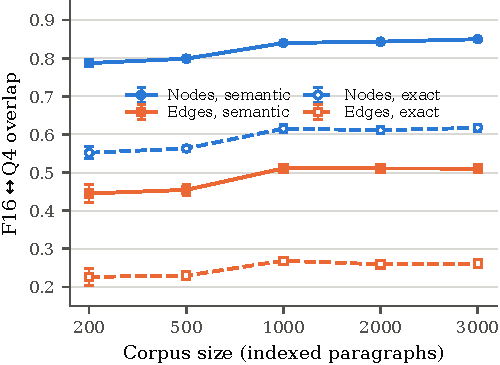
\includegraphics[width=\columnwidth]{pics/fig_overlap.pdf}
    \captionsetup{width=\columnwidth}
    \caption{Exact versus semantic agreement between the two graphs, five-seed mean $\pm$ s.d. Nodes are shown in blue and edges in orange. Solid lines require only semantic equivalence (MiniLM cosine $\geq 0.85$), dashed lines require an exact string match. The gap between a line and its dashed twin is the divergence that is pure surface form; it accounts for $52$--$61\%$ of the node disagreement and $28$--$34\%$ of the edge disagreement. All four measures rise with corpus size.}
    \label{fig:overlap}
\end{figure}


\noindent
Fig.~\ref{fig:overlap} decomposes the disagreement. Relaxing the match criterion from string identity to semantic equivalence lifts node overlap from $0.62$ to $0.85$, a gap of $23$ points that is stable across sizes, and roughly \emph{doubles} edge overlap, from $0.26$ to $0.51$. Put as a share of the apparent disagreement, semantic matching accounts for $52$--$61\%$ of it for nodes and $28$--$34\%$ for edges: that fraction is not a difference in what was extracted but in how it was spelled, one arm writing \emph{US} where the other writes \emph{United States}.

\noindent
The two edge measures answer different questions, which is why both are reported. Exact edge Jaccard counts an edge as shared only when the \emph{same ordered pair of entity labels} is linked in both graphs; it therefore requires two exact node-label matches to hold simultaneously, compounding the surface-form problem, and says nothing about how the connection is phrased. The semantic measure linearizes each edge to a \emph{source--relation--target} statement and matches on meaning, so it does test the relation phrasing. Semantic edge overlap sits below semantic node overlap because such a statement bundles two entities and a relation, leaving more that can differ than in a lone entity label. It is a strictly harder test, not evidence of worse relational knowledge.

\noindent
Every overlap measure also \emph{increases} with corpus size, and the exact and semantic curves stay roughly parallel. More documents mean more mentions per entity, and repeated mentions constrain both arms toward the same canonical form. This matters for larger indexes than the ones we built: the divergence quantization introduces does not build up as the corpus grows, it shrinks.

\begin{table*}[t]
\centering
\caption{Downstream question answering and retrieval by corpus size}
\label{tab:qa}
\footnotesize
\setlength{\tabcolsep}{6pt}
\begin{tabular}{llccccccc}
\toprule
\textbf{Size} & \textbf{Arm} & \textbf{Correctness} & \textbf{Pass@4.0} & \textbf{Cover-EM} & \textbf{Token recall} & \textbf{Hit@1} & \textbf{Hit@5} & \textbf{MRR} \\
\midrule
200 & F16 & 4.194\,$\pm$\,0.272 & 0.754\,$\pm$\,0.088 & 0.687\,$\pm$\,0.124 & 0.799\,$\pm$\,0.085 & 0.919\,$\pm$\,0.029 & 0.952\,$\pm$\,0.023 & 0.934\,$\pm$\,0.026 \\
 & Q4\_K\_M & 4.176\,$\pm$\,0.300 & 0.757\,$\pm$\,0.087 & 0.683\,$\pm$\,0.133 & 0.790\,$\pm$\,0.093 & 0.940\,$\pm$\,0.016 & 0.973\,$\pm$\,0.010 & 0.955\,$\pm$\,0.013 \\
\addlinespace[1pt]
\rowcolor{gray!10}500 & F16 & 4.010\,$\pm$\,0.272 & 0.715\,$\pm$\,0.080 & 0.659\,$\pm$\,0.129 & 0.767\,$\pm$\,0.086 & 0.898\,$\pm$\,0.005 & 0.954\,$\pm$\,0.004 & 0.922\,$\pm$\,0.004 \\
\rowcolor{gray!10} & Q4\_K\_M & 4.017\,$\pm$\,0.254 & 0.716\,$\pm$\,0.073 & 0.658\,$\pm$\,0.111 & 0.764\,$\pm$\,0.077 & 0.894\,$\pm$\,0.006 & 0.951\,$\pm$\,0.004 & 0.919\,$\pm$\,0.006 \\
\addlinespace[1pt]
1000 & F16 & 4.410\,$\pm$\,0.030 & 0.831\,$\pm$\,0.005 & 0.867\,$\pm$\,0.006 & 0.903\,$\pm$\,0.006 & 0.858\,$\pm$\,0.009 & 0.938\,$\pm$\,0.004 & 0.892\,$\pm$\,0.006 \\
 & Q4\_K\_M & 4.389\,$\pm$\,0.021 & 0.823\,$\pm$\,0.005 & 0.862\,$\pm$\,0.010 & 0.898\,$\pm$\,0.008 & 0.858\,$\pm$\,0.013 & 0.935\,$\pm$\,0.005 & 0.891\,$\pm$\,0.010 \\
\addlinespace[1pt]
\rowcolor{gray!10}2000 & F16 & 4.312\,$\pm$\,0.059 & 0.806\,$\pm$\,0.016 & 0.837\,$\pm$\,0.018 & 0.875\,$\pm$\,0.015 & 0.810\,$\pm$\,0.010 & 0.901\,$\pm$\,0.014 & 0.848\,$\pm$\,0.011 \\
\rowcolor{gray!10} & Q4\_K\_M & 4.271\,$\pm$\,0.017 & 0.794\,$\pm$\,0.004 & 0.821\,$\pm$\,0.006 & 0.865\,$\pm$\,0.007 & 0.809\,$\pm$\,0.006 & 0.899\,$\pm$\,0.002 & 0.848\,$\pm$\,0.005 \\
\addlinespace[1pt]
3000 & F16 & 4.249\,$\pm$\,0.030 & 0.788\,$\pm$\,0.006 & 0.816\,$\pm$\,0.009 & 0.861\,$\pm$\,0.007 & 0.782\,$\pm$\,0.008 & 0.884\,$\pm$\,0.006 & 0.825\,$\pm$\,0.007 \\
 & Q4\_K\_M & 4.226\,$\pm$\,0.021 & 0.782\,$\pm$\,0.006 & 0.803\,$\pm$\,0.005 & 0.852\,$\pm$\,0.004 & 0.781\,$\pm$\,0.005 & 0.883\,$\pm$\,0.005 & 0.824\,$\pm$\,0.005 \\
\bottomrule
\end{tabular}
\parbox[t]{0.95\textwidth}{\vspace{0.1cm}Five-seed mean $\pm$ standard deviation; both arms answer the identical questions over identically chunked documents and share one embedding model, so every column is a paired comparison. Correctness is the 1--5 judge score and Pass@4.0 the fraction scoring $\geq 4$. The elevated standard deviations at sizes 200 and 500 are driven by a single seed (v0) that scores far above the others in \emph{both} arms; it is retained unmodified. BERTScore-recall is omitted: it sits at $\sim$0.85 for every size and both arms (s.d.\ $\leq 0.002$) and discriminates nothing.}
\end{table*}


\section{Results II: Downstream Quality}\label{sec:qa}

\subsection{Answers and retrieval}

\noindent
Table~\ref{tab:qa} reports downstream quality. Judge correctness differs between the arms by at most $0.041$ points on the 1--5 scale, at every corpus size, and pass@4.0 by at most $0.012$. Both quantities are well inside the seed-to-seed spread. Cover-EM and token recall agree to within $0.017$ and $0.011$. BERTScore-recall is reported for completeness in the text only: it sits at $\approx 0.85$ for every size and both arms with a standard deviation $\leq 0.002$, so it separates nothing here and we do not tabulate it. Retrieval is the sharpest null of all: from size 1000 upward, Hit@5 and MRR differ between arms by less than $0.004$. This is unsurprising in hindsight and important in substance: retrieval is driven by dense embeddings from a \emph{shared} encoder over identical chunks, so the graphs' differing entity labels barely perturb which chunk surfaces.

\noindent
Table~\ref{tab:qa} has two features that bear on the comparison. First, absolute scores are not monotone in corpus size (sizes 200 and 500 score \emph{lower} than 1000), because the questions differ between size slices; only the within-row F16/Q4 contrast is a controlled comparison. Second, the standard deviations at sizes 200 and 500 are conspicuously larger than elsewhere. This is driven by a single seed (v0) whose sampled questions are markedly easier, in \emph{both} arms alike ($4.73$ and $4.55$ correctness against $\approx 4.0$ for the others). Because it moves both arms together it does not bias the paired contrast, and we retain it unmodified.

\begin{table}[t]
\centering
\caption{Paired F16 vs.\ Q4\_K\_M correctness (pooled over five seeds)}
\label{tab:paired}
\footnotesize
\setlength{\tabcolsep}{3pt}
\begin{tabular}{lcccccc}
\toprule
\textbf{Size} & $n$ & \textbf{Mean $\Delta$} & \textbf{Med.} & \textbf{Wilcoxon $p$} & \textbf{$d_z$} & \textbf{$r_{rb}$} \\
\midrule
200 & 1{,}000 & +0.0180 & 0.000 & 0.703 & +0.0121 & +0.0250 \\
\rowcolor{gray!10}500 & 2{,}500 & -0.0070 & 0.000 & 0.850 & -0.0044 & -0.0075 \\
1000 & 4{,}999 & +0.0211 & 0.000 & 0.210 & +0.0170 & +0.0443 \\
\rowcolor{gray!10}2000 & 9{,}999 & +0.0414 & 0.000 & \textbf{0.002} & +0.0307 & +0.0743 \\
3000 & 14{,}999 & +0.0226 & 0.000 & \textbf{0.046} & +0.0163 & +0.0377 \\
\bottomrule
\end{tabular}
\parbox[t]{0.485\textwidth}{\vspace{0.1cm}$\Delta$ = F16 $-$ Q4\_K\_M judge score on the same question. Two-sided Wilcoxon signed-rank test; $d_z$ is Cohen's $d$ for paired samples and $r_{rb}$ the matched-pairs rank-biserial correlation. Bold marks $p < 0.05$: it is reached only at the two largest $n$, where $|d_z| \leq 0.031$, an order of magnitude below the 0.2 conventionally called small, and the median difference is exactly zero at every size.}
\end{table}


\subsection{Paired significance}

\noindent
Table~\ref{tab:paired} pools per-question scores across seeds. The median difference is exactly zero at every size, and ties dominate: at size 3000, 11{,}316 of 14{,}999 questions receive identical scores from the two arms, with the remainder split nearly evenly (1{,}900 \fsixteen\ wins against 1{,}783 for \qfour). The Wilcoxon test returns $p > 0.2$ at sizes 200, 500, and 1000. At sizes 2000 and 3000 it returns $p = 0.0017$ and $p = 0.046$, and this is exactly the case in which a $p$-value must not be read alone. The corresponding effect sizes are $d_z = 0.031$ and $0.016$, roughly an order of magnitude below the $0.2$ conventionally called \emph{small}. What the test detects at $n \approx 10^4$ is a real but minute tilt toward \fsixteen\ of about four hundredths of a point on a five-point scale: a genuine finding about the arms' ordering, and no basis whatsoever for choosing between them.

\subsection{Structural drift does not predict downstream loss}

\begin{figure}[t]
    \centering
    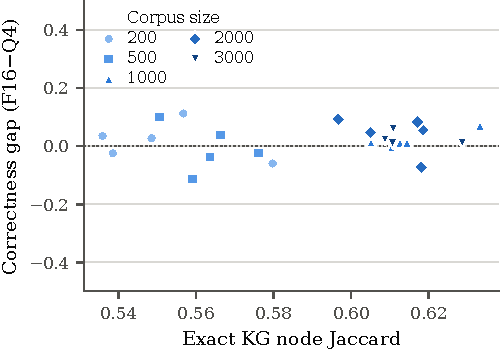
\includegraphics[width=\columnwidth]{pics/fig_decoupling.pdf}
    \captionsetup{width=\columnwidth}
    \caption{Structural drift does not predict downstream loss. Each marker is one (size, seed) run: horizontally, how much the two graphs agree node-for-node; vertically, the resulting difference in mean judge correctness on a 1--5 scale. Exact agreement ranges over eight points of Jaccard, yet every run's answer gap sits within $\pm 0.12$ of zero and the sign alternates.}
    \label{fig:decoupling}
\end{figure}


\noindent
Fig.~\ref{fig:decoupling} puts the two levels on the same axes. Across the 25 runs, exact node Jaccard varies over eight points ($0.54$ to $0.63$), yet the downstream correctness gap stays inside a narrow band around zero throughout and alternates in sign. Runs whose graphs agree least are not the runs whose answers diverge most. Structural drift, as measured by exact overlap, carries essentially no signal about downstream utility.

\begin{table}[t]
\centering
\caption{Judge correctness by node-exclusivity group}
\label{tab:nodeexcl}
\footnotesize
\setlength{\tabcolsep}{2pt}
\begin{tabular}{lcccccc}
\toprule
\textbf{Group} & $n$ & \textbf{F16} & \textbf{Q4} & \textbf{$\Delta$} & \textbf{$d_z$} & \textbf{$p$} \\
\midrule
Shared only \emph{(control)} & 20{,}067 & 4.309 & 4.279 & +0.029 & +0.022 & 0.002 \\
\rowcolor{gray!10}One from each arm & 1{,}756 & 4.343 & 4.356 & -0.013 & -0.010 & 0.643 \\
F16-only entity & 6{,}226 & 4.301 & 4.184 & +0.117 & +0.084 & 2.6e-11 \\
\rowcolor{gray!10}Q4-only entity & 4{,}562 & 4.209 & 4.320 & -0.111 & -0.079 & 7.3e-08 \\
\bottomrule
\end{tabular}
\parbox[t]{0.485\textwidth}{\vspace{0.1cm}Questions pooled over sizes 200--3000 and five seeds, grouped by whose exclusive entities they touch. Each arm answers questions about \emph{its own} exclusive entities better, by almost exactly the same margin in both directions, while the control group is flat. Exclusive entities therefore carry real information, but quantization \emph{exchanges} them rather than deleting them.}
\end{table}

\begin{figure}[t]
    \centering
    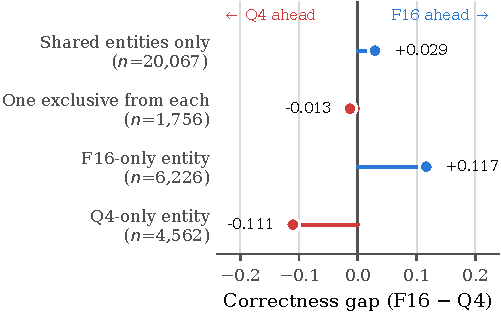
\includegraphics[width=\columnwidth]{pics/fig_nodeexcl.pdf}
    \captionsetup{width=\columnwidth}
    \caption{The model-exclusive-entity probe: judge-correctness gap by group, pooled over all sizes and seeds. Whichever arm uniquely holds an entity answers questions touching it about $0.11$ points better, and the two effects are near mirror images ($+0.117$ against $-0.111$, both $p<10^{-7}$). Questions carrying an exclusive entity from \emph{each} arm cancel out, and the shared-entity control is flat. Quantization exchanges entities rather than deleting them.}
    \label{fig:nodeexcl}
\end{figure}


\subsection{Do model-exclusive entities matter?}\label{sec:nodeexcl}

\noindent
Semantic overlap explains most of the divergence, but not all of it: each arm still holds entities with no semantic counterpart in the other. A natural worry is that these represent knowledge the quantized model genuinely lost, with the corpus-level null merely averaging it away. We test this directly. Because both arms index identical chunks and differ \emph{only} in what they extracted, the downstream effect of an entity-level difference can be isolated by grouping questions according to whose exclusive entities they touch: an \fsixteen-only entity and no \qfour-only one; a \qfour-only entity and no \fsixteen-only one; at least one exclusive entity from \emph{each} arm; or, as a no-effect anchor, only entities present in both graphs. We then compare the arms within each group, pooled over all sizes and seeds. Of 32{,}614 taggable questions, 32{,}611 joined successfully.

\noindent
The result (Table~\ref{tab:nodeexcl}, Fig.~\ref{fig:nodeexcl}) is a small, sharp, and \emph{symmetric} double dissociation. On questions touching an \fsixteen-only entity, \fsixteen\ leads by $0.117$ points; on questions touching a \qfour-only entity, \qfour\ leads by $0.111$. Both are highly significant ($p = 2.6\times10^{-11}$ and $7.3\times10^{-8}$) and the effect sizes, $|d_z| \approx 0.08$, are four to eight times the corpus-level effect. The same pattern holds in the judge-free lexical metrics, where Cover-EM shifts by $\pm 0.029$ and token recall by $+0.028$ and $-0.025$ in the matching direction, so it is not a judge artefact. Meanwhile the two flat groups are flat for different reasons: the control group has no exclusive entity to create an asymmetry ($+0.029$, the same near-zero gap seen corpus-wide), while a question carrying an exclusive entity from each arm hands each side one advantage, and they offset \emph{within} the question ($-0.013$).

\noindent
Model-exclusive entities are therefore not surface-form noise, since possessing an entity genuinely helps answer questions about it. But the advantage is small in absolute terms and, crucially, symmetric. Quantization does not delete knowledge from the graph so much as \emph{exchange} one small set of uniquely-captured entities for another of comparable value. This is the mechanism behind the corpus-level null, and it is a stronger claim than the null alone: the two effects do not merely fail to appear, they appear and cancel.

\begin{table}[t]
\centering
\caption{Index-build cost per seed (GPU hours, one A40)}
\label{tab:cost}
\footnotesize
\setlength{\tabcolsep}{5pt}
\begin{tabular}{lccc}
\toprule
\textbf{Size} & \textbf{F16 (seeds)} & \textbf{Q4\_K\_M (seeds)} & \textbf{Speed-up} \\
\midrule
200 & 1.97 (5) & 0.84 (5) & 2.34$\times$ \\
\rowcolor{gray!10}500 & 4.91 (5) & 2.22 (5) & 2.21$\times$ \\
1000 & 6.08 (5) & 4.89 (5) & 1.24$\times$ \\
\rowcolor{gray!10}2000 & 11.69 (5) & 10.27 (5) & 1.14$\times$ \\
3000 & \emph{n/a} & 16.20 (4) & -- \\
\bottomrule
\end{tabular}
\parbox[t]{0.485\textwidth}{\vspace{0.1cm}Mean wall-clock hours over the completed builds at each size, with the number of completed seeds in parentheses. \textbf{No F16 build at size 3000 completed within the 24\,h scheduler limit}, so no speed-up can be reported there. The advantage shrinks monotonically with corpus size, from $2.3\times$ to $1.1\times$: at small corpora the run is dominated by generator decoding, which Q4\_K\_M accelerates, whereas at large corpora an increasing share goes to embedding, graph merging, and I/O, which are identical in both arms. Weight memory is 15.24\,GB (F16) against 4.68\,GB (Q4\_K\_M).}
\end{table}


\subsection{Compute cost}

\noindent
Table~\ref{tab:cost} reports index-build cost. \qfour\ builds are $2.34\times$ faster at size 200 and $2.21\times$ at 500, but the advantage narrows to $1.24\times$ at 1000 and $1.14\times$ at 2000. The narrowing is expected: only generator decoding is accelerated by quantization, and its share of wall-clock time falls as embedding, entity merging, description condensation, and I/O grow with the index. We cannot report a speed-up at size 3000, because no \fsixteen\ build at that size completed inside the 24-hour scheduler limit, which is itself a cost result, if an inconveniently shaped one. The memory advantage does not decay: 4.68\,GB against 15.24\,GB of weights, the difference between fitting a 7B KG-RAG generator on a commodity 8\,GB card and not.

\begin{table}[t]
\centering
\caption{TriviaQA generalization check (single seed)}
\label{tab:trivia}
\footnotesize
\setlength{\tabcolsep}{3pt}
\begin{tabular}{lccccccccc}
\toprule
& & \multicolumn{2}{c}{\textbf{Correct.}} & \multicolumn{2}{c}{\textbf{Pass@4}} & & & \multicolumn{2}{c}{\textbf{KG ovl.}} \\
\cmidrule(lr){3-4}\cmidrule(lr){5-6}\cmidrule(lr){9-10}
\textbf{Docs} & $n$ & F16 & Q4 & F16 & Q4 & $p$ & $d_z$ & exact & sem. \\
\midrule
25 & 14 & 2.750 & 3.393 & 0.429 & 0.571 & 0.22 & -0.29 & 0.528 & 0.801 \\
\rowcolor{gray!10}50 & 28 & 3.179 & 3.804 & 0.500 & 0.643 & 0.12 & -0.30 & 0.592 & 0.841 \\
75 & 42 & 3.750 & 3.821 & 0.643 & 0.691 & 0.82 & -0.04 & 0.529 & 0.812 \\
\rowcolor{gray!10}100 & 58 & 4.086 & 3.922 & 0.724 & 0.690 & 0.47 & +0.09 & 0.556 & 0.823 \\
\bottomrule
\end{tabular}
\parbox[t]{0.485\textwidth}{\vspace{0.1cm}\textbf{Underpowered by construction}: a single seed and 14--58 questions per size. No size reaches significance and the effect sizes alternate in sign, so this establishes only that a second, harder corpus does not \emph{contradict} the SQuAD result; it cannot confirm it. \emph{Docs} counts indexed Wikipedia articles ($\sim$29 chunks each), not paragraphs. KG overlap columns are exact and semantic node overlap.}
\end{table}


\subsection{Generalization check on TriviaQA}\label{sec:trivia}

\noindent
Table~\ref{tab:trivia} reports the TriviaQA replication, which is single-seed with 14 to 58 questions per size and so underpowered by construction: it can fail to contradict the SQuAD result but cannot confirm it. It does not contradict it. No size reaches significance ($p = 0.22$, $0.12$, $0.82$, $0.47$), the effect sizes alternate in sign, and where the arms differ it is \qfour\ that leads at the smaller corpora. The graph-level picture reproduces too: exact node Jaccard $0.53$--$0.59$ against semantic node overlap $0.80$--$0.84$, the same gap seen on SQuAD, here on full Wikipedia articles rather than single paragraphs.

\noindent
Absolute scores are much lower than on SQuAD, as expected for a harder task, and retrieval in particular collapses with corpus size (gold-article Hit@5 falls from $0.71$ to $0.24$ for \fsixteen). Notably, correctness \emph{rises} over the same range ($2.75 \to 4.09$) while gold-article retrieval falls. The retrieval metric credits only the question's own evidence article, whereas the answer is generated from graph-mediated context as a whole; as the index grows, entity descriptions and relations accumulated from other articles supply enough context to answer correctly even when the gold chunk is not top-ranked. This is a property of graph-mediated retrieval, and it affects both arms identically.

\section{Discussion}\label{sec:discussion}

\subsection{Why the decoupling happens}

\noindent
Visible structural drift leaves answers unchanged for two reasons. The first is that most of the drift is not real: semantic overlap of $0.85$ against exact overlap of $0.62$ means the two graphs largely encode the same entities under different labels. The second is that the retrieval-and-answer machinery is built to absorb exactly this kind of difference. Retrieval runs on dense embeddings from a shared encoder, which match on meaning rather than on strings, and over chunks that are identical in both arms because only the extracted entities differ. An entity recorded as \emph{US} in one graph and \emph{United States} in the other pulls the same chunk into the same context and yields the same answer. The graph differences are real; they are also downstream-inert.

\noindent
That second reason is also a boundary on the claim. LightRAG's \texttt{hybrid} retrieval reaches the raw chunks as well as the graph, and those chunks are byte-identical in both arms, so chunk-level dense retrieval can recover an answer the degraded graph alone would have missed. The redundancy that makes the pipeline robust is therefore also what caps the cost of a damaged graph, and our result should be read as a statement about KG-RAG of this kind. A pipeline that answers by traversing the graph itself, such as a text-to-Cypher system, has no chunk-level fallback for a mislabelled entity or a missing edge and would plausibly be far more sensitive to the same drift. We have not tested that class of system, and the decoupling found here should not be assumed to extend to it.

\noindent
The node-exclusivity probe (Section~\ref{sec:nodeexcl}) sharpens this into a claim about the \emph{residual}, the part semantic matching does not explain. That residual is not inert: it moves answers, measurably and in the expected direction. It simply moves them both ways, in proportions that cancel. This is a more informative result than a plain null, and it predicts where the null would break: an asymmetric extraction failure, a quantized model that systematically dropped a \emph{category} of entity rather than trading one arbitrary set for another, would not cancel, and would show up here as a one-sided effect. We do not observe that at 4 bits.

\subsection{Statistical versus practical significance}

\noindent
This study requires reading the two apart. At $n \approx 15{,}000$ the Wilcoxon test detects a difference at sizes 2000 and 3000. The honest summary is not ``\fsixteen\ is better'' but ``\fsixteen\ is better by $0.04$ points out of $5$, which we can measure only because we ran fifteen thousand paired questions.'' Had we run a single seed at size 200, a common scale for RAG evaluations, we would have seen $p = 0.70$ and concluded no difference. Both readings are correct about their own evidence, and neither supports a different deployment decision. This is why we report $d_z$ and the rank-biserial correlation beside every $p$-value.

\subsection{Practical implications}

\noindent
For a practitioner building a LightRAG-style index with a 7B generator, the recommendation is unambiguous: use the 4-bit quantized model. It costs a third of the weight memory, builds the index up to $2.3\times$ faster at the corpus sizes where build time is dominated by generation, and produces a pipeline we cannot distinguish from the half-precision one on any answer or retrieval metric we measured. The one caveat is that the graphs are \emph{not} interchangeable artefacts: if the extracted graph is itself a deliverable, to be inspected, curated, merged with another knowledge base, or matched against a schema by exact entity name, then a $0.6$ node Jaccard between precisions is a real operational fact, even though it does not reach the answers.

\subsection{Limitations}

\noindent
Six limitations bound the claims. \emph{(i)} The multi-seed evidence rests on one primary dataset, SQuAD, whose short single-paragraph contexts make retrieval comparatively easy; the TriviaQA replication is a check, not a second study, and is underpowered as reported. \emph{(ii)} We compare one model family at one scale and one bit-width, so whether the decoupling survives at 2 or 3 bits, for a 1--3B generator with less redundancy to spare, or under a calibrated scheme such as GPTQ or AWQ remains open; each case means repeating the full paired design at several hundred GPU-hours. The node-exclusivity probe is the instrument for finding that breaking point, since an asymmetric loss would register there before corpus-level metrics moved. \emph{(iii)} Correctness depends on an LLM judge; we mitigate this by scoring both arms with the identical judge and by reporting judge-free lexical and retrieval measures that agree with it, but a judge-specific bias shared by both arms would be invisible to us, and we did not run a human agreement study on a sample of the judged answers, which would bound that risk directly. \emph{(iv)} Exact overlap is deliberately strict and semantic overlap depends on a threshold ($0.85$) and encoder (MiniLM); the qualitative exact-versus-semantic gap is robust, the precise values are not. \emph{(v)} Retrieval treats only the question's own gold paragraph as correct, which understates quality whenever another chunk supports the answer. This applies equally in both arms, so the comparison stands, but the absolute retrieval numbers are a lower bound. \emph{(vi)} We measure whether quantization changes the graph and whether that reaches the answers, but not how much the graph contributes in the first place relative to dense retrieval over the raw chunks; a \texttt{naive}-mode ablation re-querying these indexes with the graph bypassed is the direct test, and would calibrate how much headroom the decoupling occupies. Relatedly, SQuAD and TriviaQA questions are predominantly single-hop, and a multi-hop benchmark traversing several edges is where structural damage would most plausibly surface. Those two experiments, with a traversal-based pipeline, are what we would run next.

\section{Conclusion}\label{sec:conclusion}

\noindent
We asked whether quantizing the generator damages the knowledge graph a KG-RAG system builds, and whether any such damage reaches the answers. The answers are: yes to the first in surface form, largely no in substance, and no to the second. Four-bit \qfour\ quantization of a 7B generator produces knowledge graphs that share only $0.55$--$0.62$ of their entities and $0.23$--$0.27$ of their relations exactly with the half-precision baseline, while matching it on size, degree, connectivity, and topology, and while agreeing on $0.85$ of entities semantically. Downstream, across 33{,}497 paired questions spanning five corpus sizes and five seeds, the two pipelines are indistinguishable on judged correctness, lexical recall, and retrieval, with effect sizes an order of magnitude below the conventional small threshold even where large samples make a difference detectable. The explanation, and our central result, is that the residual entity-level differences carry a real but \emph{symmetric} effect that cancels: quantization exchanges extracted knowledge rather than destroying it. That also marks the boundary of the claim. It holds for KG-RAG whose retrieval reaches the raw chunks alongside the graph, on predominantly single-hop questions; a pipeline that answers by traversing the graph itself has no such fallback and may not be so forgiving. For roughly a third of the memory and up to $2.3\times$ faster index construction, 4-bit is a favourable default for KG-RAG of the kind we tested.

\noindent
Several experiments follow. A multi-hop benchmark and a traversal-based pipeline would test the boundary just named; a \texttt{naive}-mode ablation over these indexes would quantify how much the graph contributes at all, and an embedder ablation how much of the absorption it performs. A bit-width sweep would locate where the exchange becomes a loss, with the node-exclusivity probe as the instrument.

\bibliographystyle{IEEEtran}
\bibliography{refs}

\end{document}
